\textbf{Problem 1a: Bloch sphere form}. Consider the following single qubit state $\ket{\psi} = a_0\ket{0} + a_1\ket{1}$ where the amplitudes are given in polar form as: $(|a_0| = 0.383, \theta_0 = \pi)$ and $(|a_1| = 0.924, \theta_0 = -\pi /2)$ 
As per the definition given in the lectures, convert to Bloch sphere form specifying the Bloch angles $\theta_B$ and $\phi_B$. Plot on the Bloch sphere.


\textbf{Answer}. The Bloch sphere form of a quantum state $\ket{\psi}$ is parameterised by the angles $\theta_B$ and $\phi_B$, which respectively represent the colatitude with respect to the z-axis, and the longitude with respect to the x-axis.
\begin{align*}
	\ket{\psi} &= 0.383 \cdot e^{i \pi} \ket{0} + 0.924 \cdot e^{-i \frac{\pi}{2}} \ket{1} \\
	&= e^{i \pi} (0.383 \ket{0} + 0.924 \cdot e^{-i \frac{3\pi}{2}} \ket{1}) \\
	&= \cos(\frac{0.7498 \pi}{2}) \ket{0} + \sin(\frac{0.7498 \pi}{2}) e^{-i \frac{3\pi}{2}} \ket{1}  
\end{align*}

Thus, $\theta_B = 0.7498\pi$ and $\phi_B = -\frac{3\pi}{2}$.
$\ket{\psi}$ is visualised on the Bloch sphere below

\begin{figure}[H]
	\captionlistentry{}
	\label{fig:laissez-faire}
	\begin{center}
	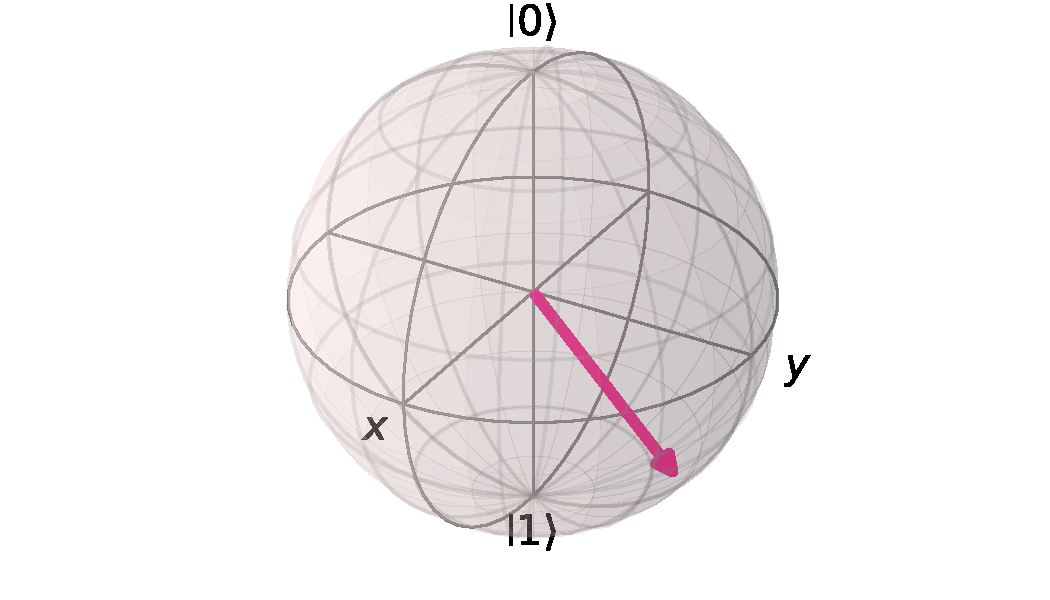
\includegraphics[width=0.85\linewidth]{graphics/q1a.pdf}
	\end{center}
    \textsf{\footnotesize{\textbf{Figure 1}: Bloch Sphere representation of $\ket{\psi} = \cos(\frac{0.7498 \pi}{2}) \ket{0} + \sin(\frac{0.7498 \pi}{2}) e^{-i \frac{3\pi}{2}} \ket{1}$}}
\end{figure}